\documentclass[12pt]{article}

\usepackage[utf8]{inputenc}
\usepackage[T2A]{fontenc}
\usepackage[english,russian]{babel}
\usepackage{amssymb}
\usepackage{graphicx}
\graphicspath{ {images/} }

\textwidth=431pt
\textheight=600pt
\hoffset=-30pt
\voffset=-30pt

\usepackage{graphicx}
\usepackage{amsmath}
\makeatletter
\renewcommand{\@oddhead}{%
\vbox{%
\hbox to \textwidth{\strut \textit{SABD, Problem set 2, Usvyatsov Mikhail} \hfill }
%\hbox to\textwidth{Лист\hfill Страница~\arabic{page}~из 2}
\hrule
\vspace{12pt}
}}
\renewcommand{\@oddfoot}{}
\makeatother


\begin{document}

%\tableofcontents

%\newpage

\begin{center}
\textbf{Problem set 2 \\
DUE: Mon. September 8, 2014 \\}
\end{center}

\newcounter{qcounter}

\bigskip
	
\textbf{Exercise 1}		
		
Compute the sample mean and standard deviation of growth and tradeshr.
\medskip
		
\textbf{Solution}

E(growth) = 1.9427
E(tradeshr) = 0.5647

$\sigma(growth) = 1.37736$
$\sigma(tradeshr) = 0.5378386$
\bigskip

\textbf{Exercise 2}
		
Estimate a regression of growth on tradeshr, using the “robust” option.

\begin{list}{\alph{qcounter})~}{\usecounter{qcounter}}
\item
What is the coefficient on tradeshr? Explain in words what it means. Is the numerical value of your estimate large or small in an economic (real-world) sense?
\item
Graph the data points and the estimated regression line.
\item
Is the slope coefficient statistically significantly different from zero at the 5\% significance level? Show how you reach this conclusion.
\item
Report the 95\% confidence interval for $\beta_1$ , the slope of the population regression line.
\item
What is the $R^2$ of this regression? What does this mean?
\item
Compute the correlation coefficient between growth and tradeshr, and compare its square to the $R^2$. How are the correlation coefficient and the $R^2$ related?
\item
What is the value of the root mean squared error of the regression? What does this mean?
\item
Based on your graph from (b), does the regression error appear to be homoskedastic or heteroskedastic?
\item
Run the regression again without the “robust” option. Compare the results to what you obtained with the “robust” option. What is different?
\item
You should see an outlier in the data set. Rerun the regression (with the “robust” option), dropping the outlier. Does dropping the outlier make a qualitative difference to your results? Explain.
\item
What is the outlying observation? Considering the economics of the relation you are investigating, in your judgment should that outlier be omitted from the regression? (You might need to do a bit of research about that outlier to answer this question properly.)
\end{list}
\medskip
		
\textbf{Solution}

\begin{list}{\alph{qcounter})~}{\usecounter{qcounter}}
\item
The slope coefficient on tradeshr is 2.2233374. It means that if tradeshr will be changed by one, growth will be changed in 2.2233374. I personally think that such value of slope parameter is large in a real-world sense.
\item
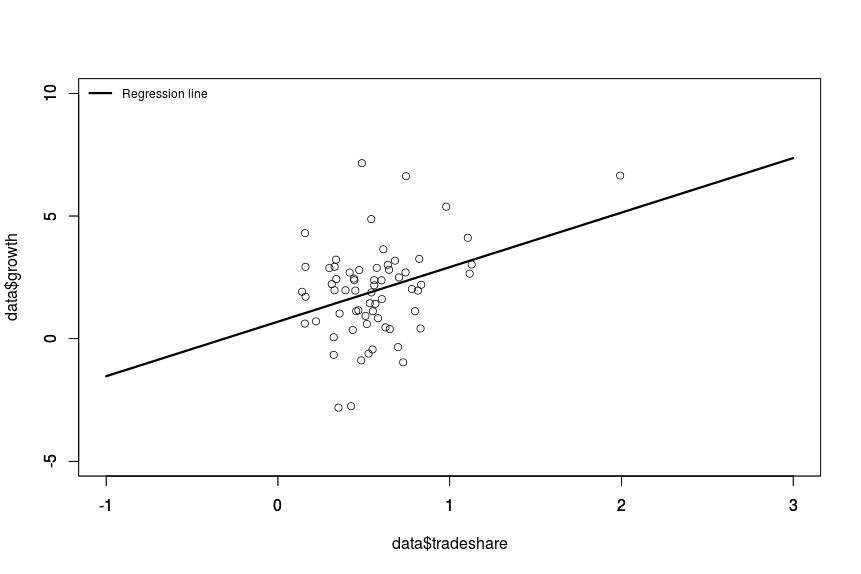
\includegraphics[width=1\textwidth]{Rplot.png}
\item
$t = \dfrac{\hat{\beta} - \beta_{1.0}}{SE(\hat{\beta})}$\\
$\beta_{1.0} = 0$\\
${SE(\hat{\beta})} = \sqrt{\hat{\sigma}^2_{\hat{\beta}}}$\\
$\hat{\sigma}^2_{\hat{\beta}} = \dfrac{1}{n} * \dfrac{\dfrac{1}{n-2} * \sum^{n}_{i = 1}(X_i - \overline{X})^2\hat{u}^2}{\left[\dfrac{1}{n} * \sum^{n}_{i = 1}(X_i-\overline{X})^2\right]^2}$\\
t = 3.221527 
t > 1.96, so we have to reject $H_0$
\item
$[\hat{\beta}_1 - 1.96*SE(\hat{\beta}_1),\hat{\beta}_1 + 1.96*SE(\hat{\beta}_1)] = [0.870643,3.576032]$
\item
$R^2 = \dfrac{ESS}{TSS} = \dfrac{\sum^{n}_{i=1}(\hat{Y}_i-\overline{Y})^2}{\sum^{n}_{i=1}(Y_i-\overline{Y})^2}=0.1149446$\\
It means that the regression on tradeshare predicts growth bad.
\item
$(corr(growth, tradeshare))^2 = 0.1236802$\\
As $R^2$
it shows that the value of tradeshare is not very much correlated with growth, however we cannot say that this values are not correlated.
\item
RMSE = $\sqrt{\dfrac{\sum^{n}_{i=1}\hat{u}^2_i}{n}}	$
\item
It seems to be heteroskedastic.
\item
According to the graphic of regressions, regression without robustness has a little bit different coefficients.
\item
According to the graphic of regressions, regression without the outlier has very different coefficients.
\item
Outlying observation is Malta. We have to omit the outlier because linear regression is sensitive for it.
\end{list}

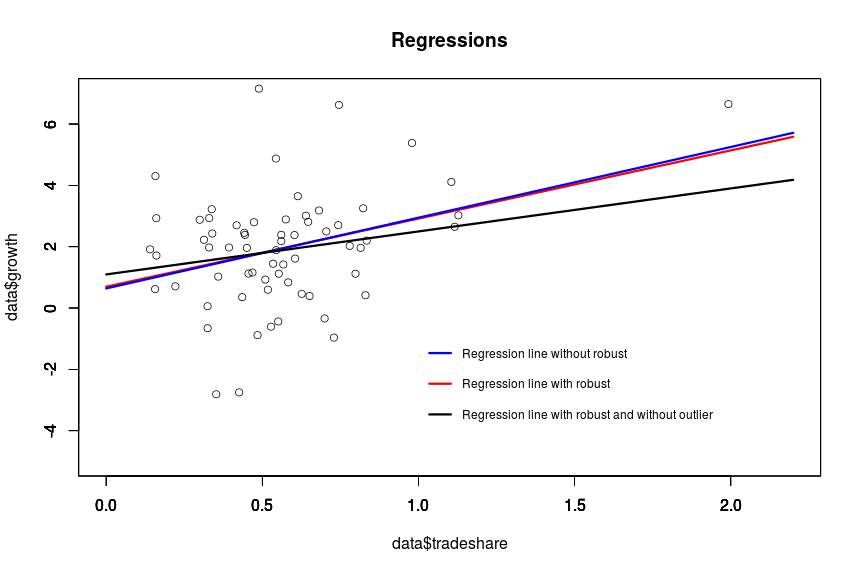
\includegraphics[width=1\textwidth]{Rplot1.png}

\textbf{Exercise 4}
\bigskip

Table 2 presents the results of three regressions, one in each column. Estimate the indicated regressions and fill in the values (you may either handwrite or type the entries in, at you convenience; if you choose to type up the table, an electronic copy of Table 2 in .doc format is available on the course Web site). For example, to fill in column (1), estimate the regression with growth as the dependent variable and tradeshr and school60 as the independent variables, using the “robust” option, and fill in the estimated coefficients and standard errors; also compute and fill in the value of the F-statistic and p-value testing the hypothesis that the coefficients on tradeshr and school60 are both zero. The adjusted $R^2$ can be computed by rerunning this regression without the “robust” option. Note: the regressions in Table 2 all exclude the observation on Malta.\\

\textbf{Solution}
\medskip

\begin{tabular}{| l | c | c |r |}
  \hline
  {\bf Regressor} & {\bf (1)} & {\bf (2)} & {\bf (3)}\\ \hline
  tradeshare & (1.5412032) & (1.3686513435) & (0.8505190649)\\ \hline
  school60 & (0.2105808) & (0.4730324670) & (0.4478457993)\\ \hline
  capstock60 & - & (-0.0003034976) & (-0.0003690296)\\ \hline
  revc & - & - & (-2.7211122223)\\ \hline
  civil & - & - & ( 0.3973022112)\\ \hline
  Intercept & 0.0972978 & 0.1509167230 & 1.0709842944 \\ \hline
  
   \multicolumn{4}{|p{15cm}|}{\bf F-statistics testing the hypothesis that the population coefficients on the indicated regressors are all zero:}  \\ \hline
  tradeshare, school60 & (4.152) & (5.5003) & (4.6298)\\ \hline
  tradeshare, school60, capstock60 & - & (3.9728) & ( 3.0852)\\ \hline
  revc, civil & - & - & (5.1212)\\ \hline
  \multicolumn{4}{|l|}{\bf Regression summary statistics}  \\ \hline
  $\overline{R^2}$  & 0.1331  & 0.2078   &0.23  \\ \hline
  $R^2$ & 0.1606 & 0.2455 &0.2911 \\ \hline
  Regression RMSE & 1.65775 & 1.572138 & 1.534965\\ \hline
  n & 64  & 64  & 64 \\ \hline
\end{tabular}

\end{document}